\documentclass[tikz,border=9pt]{standalone}
\usepackage{amsmath,amssymb}
\usetikzlibrary{arrows.meta,positioning,calc}
\begin{document}
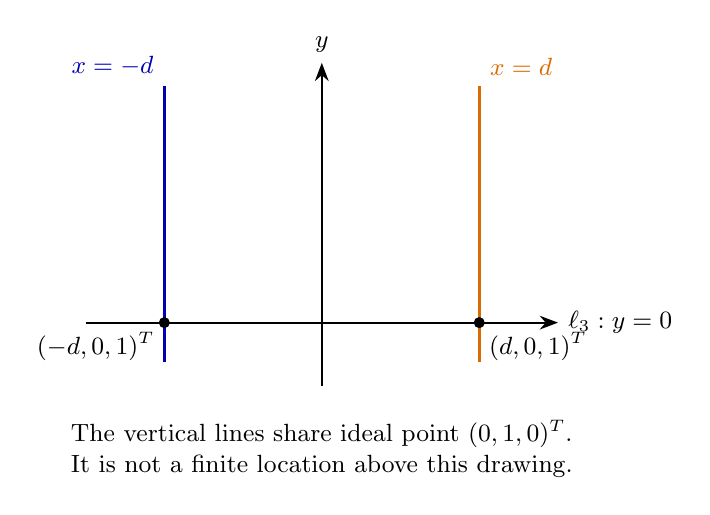
\begin{tikzpicture}[font=\small,arr/.style={-{Stealth},thick},box/.style={draw=blue!55!black,rounded corners,fill=blue!4,align=center,text width=2.9cm,minimum height=1.05cm}]

\draw[arr] (-3,0)--(3,0) node[right]{$\ell_3:y=0$};
\draw[arr] (0,-.8)--(0,3.3) node[above]{$y$};
\draw[very thick,blue!70!black] (-2,-.5)--(-2,3) node[above left]{$x=-d$};
\draw[very thick,orange!85!black] (2,-.5)--(2,3) node[above right]{$x=d$};
\fill (-2,0) circle(2pt) node[below left]{$(-d,0,1)^T$};
\fill (2,0) circle(2pt) node[below right]{$(d,0,1)^T$};
\node[align=center] at (0,-1.6){The vertical lines share ideal point $(0,1,0)^T$.\\It is not a finite location above this drawing.};

\end{tikzpicture}
\end{document}
